% 2018 天津理科第17题：空间几何示意，按原卷线型描绘。
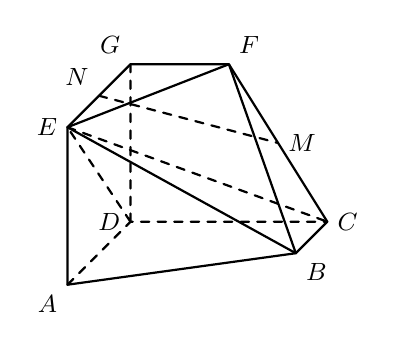
\begin{tikzpicture}[line cap=round,line join=round,thick,every node/.style={font=\small}]
  \coordinate (A) at (0,0);
  \coordinate (D) at (.8,.8);
  \coordinate (C) at (3.3,.8);
  \coordinate (B) at (2.9,.4);
  \coordinate (E) at (0,2);
  \coordinate (G) at (.8,2.8);
  \coordinate (F) at (2.05,2.8);
  % Solid visible outer edges.
  \draw (A)--(B)--(C)--(F)--(G)--(E)--(A);
  \draw (E)--(F) (F)--(B) (E)--(B);
  % Midpoints shown on the upper/rear edges.
  \coordinate (N) at (.4,2.4);
  \coordinate (M) at (2.675,1.8);
  % Rear/under edges and construction lines hidden in the source.
  \draw[dashed] (A)--(D)--(C) (D)--(G) (D)--(E);
  \draw[dashed] (E)--(C) (N)--(M);
  \node[below left] at (A) {$A$};
  \node[below right] at (B) {$B$};
  \node[right] at (C) {$C$};
  \node[left] at (D) {$D$};
  \node[left] at (E) {$E$};
  \node[above left] at (G) {$G$};
  \node[above right] at (F) {$F$};
  \node[above left] at (N) {$N$};
  \node[right] at (M) {$M$};
\end{tikzpicture}
